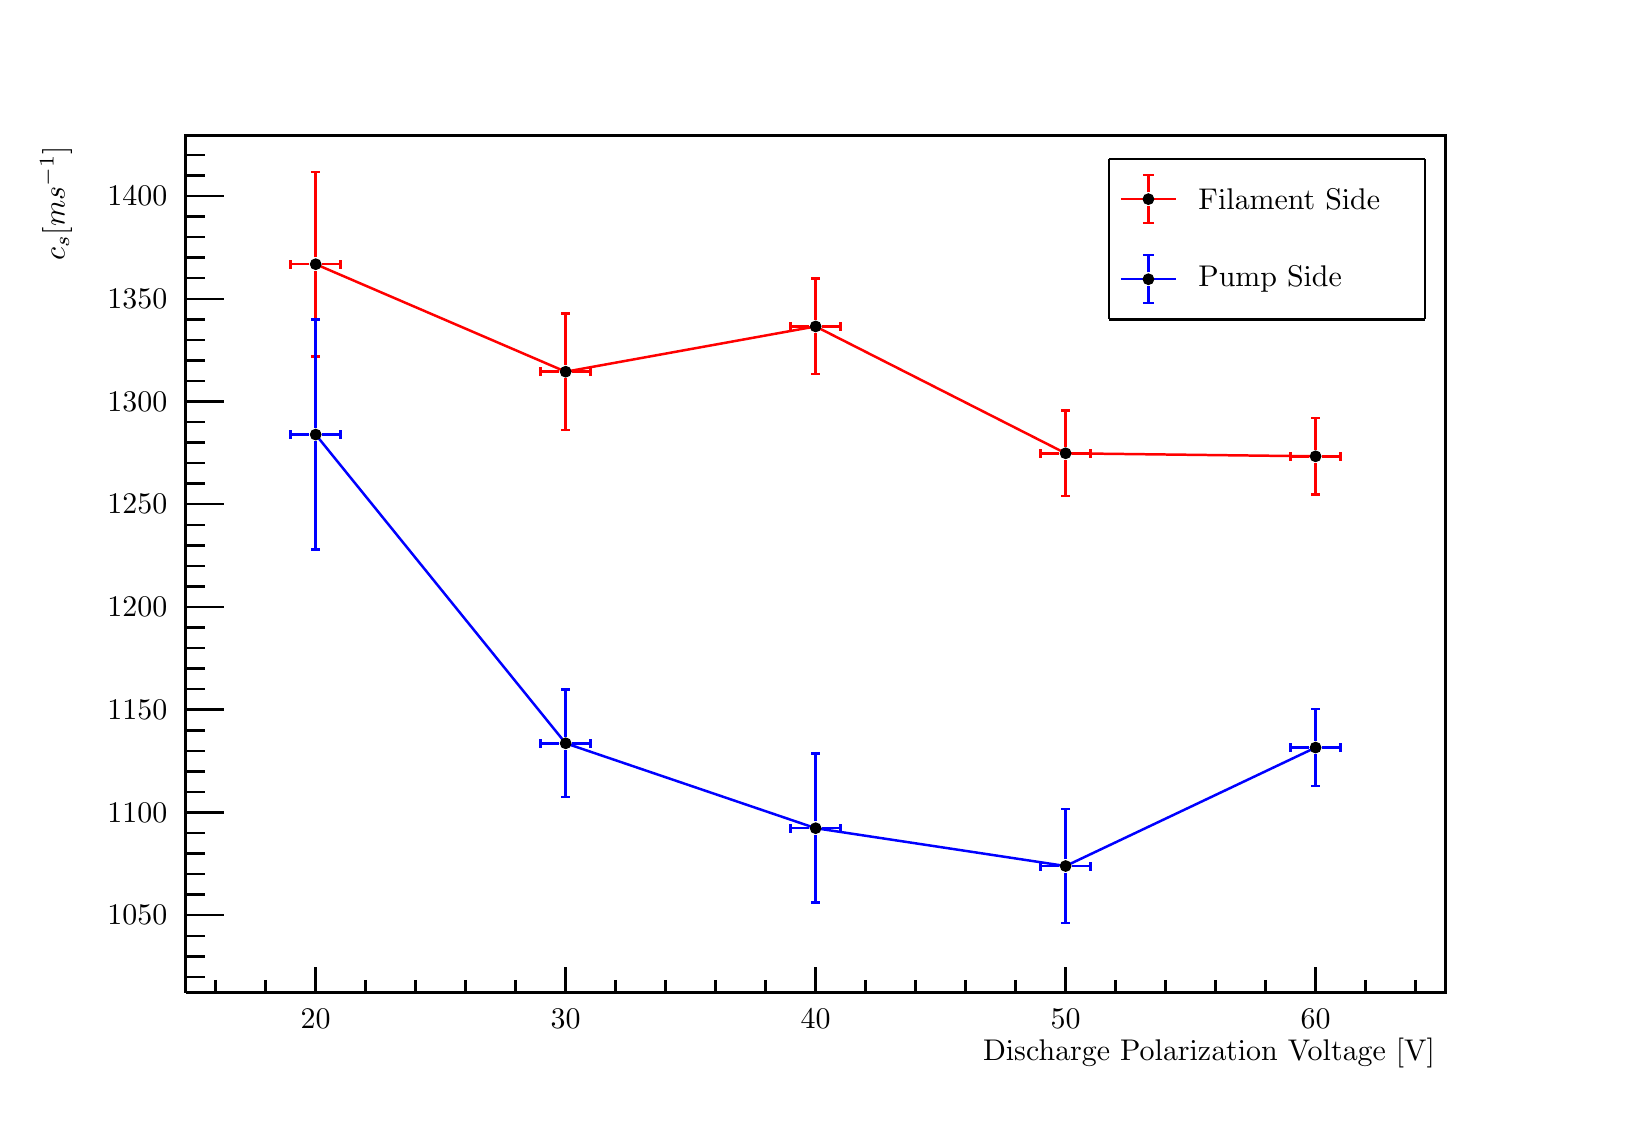
\begin{tikzpicture}
\pgfdeclareplotmark{cross} {
\pgfpathmoveto{\pgfpoint{-0.3\pgfplotmarksize}{\pgfplotmarksize}}
\pgfpathlineto{\pgfpoint{+0.3\pgfplotmarksize}{\pgfplotmarksize}}
\pgfpathlineto{\pgfpoint{+0.3\pgfplotmarksize}{0.3\pgfplotmarksize}}
\pgfpathlineto{\pgfpoint{+1\pgfplotmarksize}{0.3\pgfplotmarksize}}
\pgfpathlineto{\pgfpoint{+1\pgfplotmarksize}{-0.3\pgfplotmarksize}}
\pgfpathlineto{\pgfpoint{+0.3\pgfplotmarksize}{-0.3\pgfplotmarksize}}
\pgfpathlineto{\pgfpoint{+0.3\pgfplotmarksize}{-1.\pgfplotmarksize}}
\pgfpathlineto{\pgfpoint{-0.3\pgfplotmarksize}{-1.\pgfplotmarksize}}
\pgfpathlineto{\pgfpoint{-0.3\pgfplotmarksize}{-0.3\pgfplotmarksize}}
\pgfpathlineto{\pgfpoint{-1.\pgfplotmarksize}{-0.3\pgfplotmarksize}}
\pgfpathlineto{\pgfpoint{-1.\pgfplotmarksize}{0.3\pgfplotmarksize}}
\pgfpathlineto{\pgfpoint{-0.3\pgfplotmarksize}{0.3\pgfplotmarksize}}
\pgfpathclose
\pgfusepathqstroke
}
\pgfdeclareplotmark{cross*} {
\pgfpathmoveto{\pgfpoint{-0.3\pgfplotmarksize}{\pgfplotmarksize}}
\pgfpathlineto{\pgfpoint{+0.3\pgfplotmarksize}{\pgfplotmarksize}}
\pgfpathlineto{\pgfpoint{+0.3\pgfplotmarksize}{0.3\pgfplotmarksize}}
\pgfpathlineto{\pgfpoint{+1\pgfplotmarksize}{0.3\pgfplotmarksize}}
\pgfpathlineto{\pgfpoint{+1\pgfplotmarksize}{-0.3\pgfplotmarksize}}
\pgfpathlineto{\pgfpoint{+0.3\pgfplotmarksize}{-0.3\pgfplotmarksize}}
\pgfpathlineto{\pgfpoint{+0.3\pgfplotmarksize}{-1.\pgfplotmarksize}}
\pgfpathlineto{\pgfpoint{-0.3\pgfplotmarksize}{-1.\pgfplotmarksize}}
\pgfpathlineto{\pgfpoint{-0.3\pgfplotmarksize}{-0.3\pgfplotmarksize}}
\pgfpathlineto{\pgfpoint{-1.\pgfplotmarksize}{-0.3\pgfplotmarksize}}
\pgfpathlineto{\pgfpoint{-1.\pgfplotmarksize}{0.3\pgfplotmarksize}}
\pgfpathlineto{\pgfpoint{-0.3\pgfplotmarksize}{0.3\pgfplotmarksize}}
\pgfpathclose
\pgfusepathqfillstroke
}
\pgfdeclareplotmark{newstar} {
\pgfpathmoveto{\pgfqpoint{0pt}{\pgfplotmarksize}}
\pgfpathlineto{\pgfqpointpolar{44}{0.5\pgfplotmarksize}}
\pgfpathlineto{\pgfqpointpolar{18}{\pgfplotmarksize}}
\pgfpathlineto{\pgfqpointpolar{-20}{0.5\pgfplotmarksize}}
\pgfpathlineto{\pgfqpointpolar{-54}{\pgfplotmarksize}}
\pgfpathlineto{\pgfqpointpolar{-90}{0.5\pgfplotmarksize}}
\pgfpathlineto{\pgfqpointpolar{234}{\pgfplotmarksize}}
\pgfpathlineto{\pgfqpointpolar{198}{0.5\pgfplotmarksize}}
\pgfpathlineto{\pgfqpointpolar{162}{\pgfplotmarksize}}
\pgfpathlineto{\pgfqpointpolar{134}{0.5\pgfplotmarksize}}
\pgfpathclose
\pgfusepathqstroke
}
\pgfdeclareplotmark{newstar*} {
\pgfpathmoveto{\pgfqpoint{0pt}{\pgfplotmarksize}}
\pgfpathlineto{\pgfqpointpolar{44}{0.5\pgfplotmarksize}}
\pgfpathlineto{\pgfqpointpolar{18}{\pgfplotmarksize}}
\pgfpathlineto{\pgfqpointpolar{-20}{0.5\pgfplotmarksize}}
\pgfpathlineto{\pgfqpointpolar{-54}{\pgfplotmarksize}}
\pgfpathlineto{\pgfqpointpolar{-90}{0.5\pgfplotmarksize}}
\pgfpathlineto{\pgfqpointpolar{234}{\pgfplotmarksize}}
\pgfpathlineto{\pgfqpointpolar{198}{0.5\pgfplotmarksize}}
\pgfpathlineto{\pgfqpointpolar{162}{\pgfplotmarksize}}
\pgfpathlineto{\pgfqpointpolar{134}{0.5\pgfplotmarksize}}
\pgfpathclose
\pgfusepathqfillstroke
}
\definecolor{c}{rgb}{1,1,1};
\draw [color=c, fill=c] (0,0) rectangle (20,13.6103);
\draw [color=c, fill=c] (2,1.36103) rectangle (18,12.2493);
\definecolor{c}{rgb}{0,0,0};
\draw [c,line width=0.9] (2,1.36103) -- (2,12.2493) -- (18,12.2493) -- (18,1.36103) -- (2,1.36103);
\definecolor{c}{rgb}{1,1,1};
\draw [color=c, fill=c] (2,1.36103) rectangle (18,12.2493);
\definecolor{c}{rgb}{0,0,0};
\draw [c,line width=0.9] (2,1.36103) -- (2,12.2493) -- (18,12.2493) -- (18,1.36103) -- (2,1.36103);
\draw [c,line width=0.9] (2,1.36103) -- (18,1.36103);
\draw [c,line width=0.9] (3.65079,1.68768) -- (3.65079,1.36103);
\draw [c,line width=0.9] (4.28571,1.52436) -- (4.28571,1.36103);
\draw [c,line width=0.9] (4.92064,1.52436) -- (4.92064,1.36103);
\draw [c,line width=0.9] (5.55556,1.52436) -- (5.55556,1.36103);
\draw [c,line width=0.9] (6.19048,1.52436) -- (6.19048,1.36103);
\draw [c,line width=0.9] (6.8254,1.68768) -- (6.8254,1.36103);
\draw [c,line width=0.9] (7.46032,1.52436) -- (7.46032,1.36103);
\draw [c,line width=0.9] (8.09524,1.52436) -- (8.09524,1.36103);
\draw [c,line width=0.9] (8.73016,1.52436) -- (8.73016,1.36103);
\draw [c,line width=0.9] (9.36508,1.52436) -- (9.36508,1.36103);
\draw [c,line width=0.9] (10,1.68768) -- (10,1.36103);
\draw [c,line width=0.9] (10.6349,1.52436) -- (10.6349,1.36103);
\draw [c,line width=0.9] (11.2698,1.52436) -- (11.2698,1.36103);
\draw [c,line width=0.9] (11.9048,1.52436) -- (11.9048,1.36103);
\draw [c,line width=0.9] (12.5397,1.52436) -- (12.5397,1.36103);
\draw [c,line width=0.9] (13.1746,1.68768) -- (13.1746,1.36103);
\draw [c,line width=0.9] (13.8095,1.52436) -- (13.8095,1.36103);
\draw [c,line width=0.9] (14.4444,1.52436) -- (14.4444,1.36103);
\draw [c,line width=0.9] (15.0794,1.52436) -- (15.0794,1.36103);
\draw [c,line width=0.9] (15.7143,1.52436) -- (15.7143,1.36103);
\draw [c,line width=0.9] (16.3492,1.68768) -- (16.3492,1.36103);
\draw [c,line width=0.9] (3.65079,1.68768) -- (3.65079,1.36103);
\draw [c,line width=0.9] (3.01587,1.52436) -- (3.01587,1.36103);
\draw [c,line width=0.9] (2.38095,1.52436) -- (2.38095,1.36103);
\draw [c,line width=0.9] (16.3492,1.68768) -- (16.3492,1.36103);
\draw [c,line width=0.9] (16.9841,1.52436) -- (16.9841,1.36103);
\draw [c,line width=0.9] (17.619,1.52436) -- (17.619,1.36103);
\draw [anchor=base] (3.65079,0.911891) node[scale=1.08185, color=c, rotate=0]{20};
\draw [anchor=base] (6.8254,0.911891) node[scale=1.08185, color=c, rotate=0]{30};
\draw [anchor=base] (10,0.911891) node[scale=1.08185, color=c, rotate=0]{40};
\draw [anchor=base] (13.1746,0.911891) node[scale=1.08185, color=c, rotate=0]{50};
\draw [anchor=base] (16.3492,0.911891) node[scale=1.08185, color=c, rotate=0]{60};
\draw [anchor= east] (18,0.598854) node[scale=1.08185, color=c, rotate=0]{Discharge Polarization Voltage [V]};
\draw [c,line width=0.9] (2,1.36103) -- (2,12.2493);
\draw [c,line width=0.9] (2.48,2.34573) -- (2,2.34573);
\draw [c,line width=0.9] (2.24,2.6067) -- (2,2.6067);
\draw [c,line width=0.9] (2.24,2.86766) -- (2,2.86766);
\draw [c,line width=0.9] (2.24,3.12862) -- (2,3.12862);
\draw [c,line width=0.9] (2.24,3.38959) -- (2,3.38959);
\draw [c,line width=0.9] (2.48,3.65055) -- (2,3.65055);
\draw [c,line width=0.9] (2.24,3.91151) -- (2,3.91151);
\draw [c,line width=0.9] (2.24,4.17248) -- (2,4.17248);
\draw [c,line width=0.9] (2.24,4.43344) -- (2,4.43344);
\draw [c,line width=0.9] (2.24,4.6944) -- (2,4.6944);
\draw [c,line width=0.9] (2.48,4.95537) -- (2,4.95537);
\draw [c,line width=0.9] (2.24,5.21633) -- (2,5.21633);
\draw [c,line width=0.9] (2.24,5.47729) -- (2,5.47729);
\draw [c,line width=0.9] (2.24,5.73825) -- (2,5.73825);
\draw [c,line width=0.9] (2.24,5.99922) -- (2,5.99922);
\draw [c,line width=0.9] (2.48,6.26018) -- (2,6.26018);
\draw [c,line width=0.9] (2.24,6.52114) -- (2,6.52114);
\draw [c,line width=0.9] (2.24,6.78211) -- (2,6.78211);
\draw [c,line width=0.9] (2.24,7.04307) -- (2,7.04307);
\draw [c,line width=0.9] (2.24,7.30403) -- (2,7.30403);
\draw [c,line width=0.9] (2.48,7.565) -- (2,7.565);
\draw [c,line width=0.9] (2.24,7.82596) -- (2,7.82596);
\draw [c,line width=0.9] (2.24,8.08692) -- (2,8.08692);
\draw [c,line width=0.9] (2.24,8.34789) -- (2,8.34789);
\draw [c,line width=0.9] (2.24,8.60885) -- (2,8.60885);
\draw [c,line width=0.9] (2.48,8.86981) -- (2,8.86981);
\draw [c,line width=0.9] (2.24,9.13078) -- (2,9.13078);
\draw [c,line width=0.9] (2.24,9.39174) -- (2,9.39174);
\draw [c,line width=0.9] (2.24,9.6527) -- (2,9.6527);
\draw [c,line width=0.9] (2.24,9.91366) -- (2,9.91366);
\draw [c,line width=0.9] (2.48,10.1746) -- (2,10.1746);
\draw [c,line width=0.9] (2.24,10.4356) -- (2,10.4356);
\draw [c,line width=0.9] (2.24,10.6966) -- (2,10.6966);
\draw [c,line width=0.9] (2.24,10.9575) -- (2,10.9575);
\draw [c,line width=0.9] (2.24,11.2185) -- (2,11.2185);
\draw [c,line width=0.9] (2.48,11.4794) -- (2,11.4794);
\draw [c,line width=0.9] (2.48,2.34573) -- (2,2.34573);
\draw [c,line width=0.9] (2.24,2.08477) -- (2,2.08477);
\draw [c,line width=0.9] (2.24,1.82381) -- (2,1.82381);
\draw [c,line width=0.9] (2.24,1.56285) -- (2,1.56285);
\draw [c,line width=0.9] (2.48,11.4794) -- (2,11.4794);
\draw [c,line width=0.9] (2.24,11.7404) -- (2,11.7404);
\draw [c,line width=0.9] (2.24,12.0014) -- (2,12.0014);
\draw [anchor= east] (1.9,2.34573) node[scale=1.08185, color=c, rotate=0]{1050};
\draw [anchor= east] (1.9,3.65055) node[scale=1.08185, color=c, rotate=0]{1100};
\draw [anchor= east] (1.9,4.95537) node[scale=1.08185, color=c, rotate=0]{1150};
\draw [anchor= east] (1.9,6.26018) node[scale=1.08185, color=c, rotate=0]{1200};
\draw [anchor= east] (1.9,7.565) node[scale=1.08185, color=c, rotate=0]{1250};
\draw [anchor= east] (1.9,8.86981) node[scale=1.08185, color=c, rotate=0]{1300};
\draw [anchor= east] (1.9,10.1746) node[scale=1.08185, color=c, rotate=0]{1350};
\draw [anchor= east] (1.9,11.4794) node[scale=1.08185, color=c, rotate=0]{1400};
\draw [anchor= east] (0.354441,12.2493) node[scale=1.08185, color=c, rotate=90]{$c_s [m s^{-1}]$};
\definecolor{c}{rgb}{1,0,0};
\draw [c,line width=0.9] (3.65079,10.6133) -- (6.8254,9.24795) -- (10,9.82285) -- (13.1746,8.21192) -- (16.3492,8.17356);
\definecolor{c}{rgb}{0,0,0};
\foreach \P in {(3.65079,10.6133), (6.8254,9.24795), (10,9.82285), (13.1746,8.21192), (16.3492,8.17356)}{\draw[mark options={color=c,fill=c},mark size=1.921922pt,mark=*] plot coordinates {\P};}
\definecolor{c}{rgb}{1,0,0};
\draw [c,line width=0.9] (3.56483,10.6133) -- (3.33333,10.6133);
\draw [c,line width=0.9] (3.33333,10.556) -- (3.33333,10.6706);
\draw [c,line width=0.9] (3.73675,10.6133) -- (3.96825,10.6133);
\draw [c,line width=0.9] (3.96825,10.556) -- (3.96825,10.6706);
\draw [c,line width=0.9] (3.65079,10.6993) -- (3.65079,11.7867);
\draw [c,line width=0.9] (3.59349,11.7867) -- (3.7081,11.7867);
\draw [c,line width=0.9] (3.65079,10.5273) -- (3.65079,9.43991);
\draw [c,line width=0.9] (3.59349,9.43991) -- (3.7081,9.43991);
\draw [c,line width=0.9] (6.73944,9.24795) -- (6.50794,9.24795);
\draw [c,line width=0.9] (6.50794,9.19064) -- (6.50794,9.30525);
\draw [c,line width=0.9] (6.91136,9.24795) -- (7.14286,9.24795);
\draw [c,line width=0.9] (7.14286,9.19064) -- (7.14286,9.30525);
\draw [c,line width=0.9] (6.8254,9.33391) -- (6.8254,9.98641);
\draw [c,line width=0.9] (6.76809,9.98641) -- (6.8827,9.98641);
\draw [c,line width=0.9] (6.8254,9.16199) -- (6.8254,8.50948);
\draw [c,line width=0.9] (6.76809,8.50948) -- (6.8827,8.50948);
\draw [c,line width=0.9] (9.91404,9.82285) -- (9.68254,9.82285);
\draw [c,line width=0.9] (9.68254,9.76554) -- (9.68254,9.88016);
\draw [c,line width=0.9] (10.086,9.82285) -- (10.3175,9.82285);
\draw [c,line width=0.9] (10.3175,9.76554) -- (10.3175,9.88016);
\draw [c,line width=0.9] (10,9.90881) -- (10,10.4294);
\draw [c,line width=0.9] (9.94269,10.4294) -- (10.0573,10.4294);
\draw [c,line width=0.9] (10,9.73689) -- (10,9.21627);
\draw [c,line width=0.9] (9.94269,9.21627) -- (10.0573,9.21627);
\draw [c,line width=0.9] (13.0886,8.21192) -- (12.8571,8.21192);
\draw [c,line width=0.9] (12.8571,8.15462) -- (12.8571,8.26923);
\draw [c,line width=0.9] (13.2606,8.21192) -- (13.4921,8.21192);
\draw [c,line width=0.9] (13.4921,8.15462) -- (13.4921,8.26923);
\draw [c,line width=0.9] (13.1746,8.29788) -- (13.1746,8.7524);
\draw [c,line width=0.9] (13.1173,8.7524) -- (13.2319,8.7524);
\draw [c,line width=0.9] (13.1746,8.12596) -- (13.1746,7.67145);
\draw [c,line width=0.9] (13.1173,7.67145) -- (13.2319,7.67145);
\draw [c,line width=0.9] (16.2632,8.17356) -- (16.0317,8.17356);
\draw [c,line width=0.9] (16.0317,8.11626) -- (16.0317,8.23087);
\draw [c,line width=0.9] (16.4352,8.17356) -- (16.6667,8.17356);
\draw [c,line width=0.9] (16.6667,8.11626) -- (16.6667,8.23087);
\draw [c,line width=0.9] (16.3492,8.25952) -- (16.3492,8.65779);
\draw [c,line width=0.9] (16.2919,8.65779) -- (16.4065,8.65779);
\draw [c,line width=0.9] (16.3492,8.0876) -- (16.3492,7.68933);
\draw [c,line width=0.9] (16.2919,7.68933) -- (16.4065,7.68933);
\definecolor{c}{rgb}{0,0,1};
\draw [c,line width=0.9] (3.56483,8.44966) -- (3.33333,8.44966);
\draw [c,line width=0.9] (3.33333,8.39235) -- (3.33333,8.50697);
\draw [c,line width=0.9] (3.73675,8.44966) -- (3.96825,8.44966);
\draw [c,line width=0.9] (3.96825,8.39235) -- (3.96825,8.50697);
\draw [c,line width=0.9] (3.65079,8.53562) -- (3.65079,9.90844);
\draw [c,line width=0.9] (3.59349,9.90844) -- (3.7081,9.90844);
\draw [c,line width=0.9] (3.65079,8.3637) -- (3.65079,6.99089);
\draw [c,line width=0.9] (3.59349,6.99089) -- (3.7081,6.99089);
\draw [c,line width=0.9] (6.73944,4.52895) -- (6.50794,4.52895);
\draw [c,line width=0.9] (6.50794,4.47165) -- (6.50794,4.58626);
\draw [c,line width=0.9] (6.91136,4.52895) -- (7.14286,4.52895);
\draw [c,line width=0.9] (7.14286,4.47165) -- (7.14286,4.58626);
\draw [c,line width=0.9] (6.8254,4.61491) -- (6.8254,5.21185);
\draw [c,line width=0.9] (6.76809,5.21185) -- (6.8827,5.21185);
\draw [c,line width=0.9] (6.8254,4.44299) -- (6.8254,3.84606);
\draw [c,line width=0.9] (6.76809,3.84606) -- (6.8827,3.84606);
\draw [c,line width=0.9] (9.91404,3.45065) -- (9.68254,3.45065);
\draw [c,line width=0.9] (9.68254,3.39335) -- (9.68254,3.50796);
\draw [c,line width=0.9] (10.086,3.45065) -- (10.3175,3.45065);
\draw [c,line width=0.9] (10.3175,3.39335) -- (10.3175,3.50796);
\draw [c,line width=0.9] (10,3.53661) -- (10,4.39653);
\draw [c,line width=0.9] (9.94269,4.39653) -- (10.0573,4.39653);
\draw [c,line width=0.9] (10,3.36469) -- (10,2.50477);
\draw [c,line width=0.9] (9.94269,2.50477) -- (10.0573,2.50477);
\draw [c,line width=0.9] (13.0886,2.97022) -- (12.8571,2.97022);
\draw [c,line width=0.9] (12.8571,2.91291) -- (12.8571,3.02753);
\draw [c,line width=0.9] (13.2606,2.97022) -- (13.4921,2.97022);
\draw [c,line width=0.9] (13.4921,2.91291) -- (13.4921,3.02753);
\draw [c,line width=0.9] (13.1746,3.05618) -- (13.1746,3.69444);
\draw [c,line width=0.9] (13.1173,3.69444) -- (13.2319,3.69444);
\draw [c,line width=0.9] (13.1746,2.88426) -- (13.1746,2.24599);
\draw [c,line width=0.9] (13.1173,2.24599) -- (13.2319,2.24599);
\draw [c,line width=0.9] (16.2632,4.47467) -- (16.0317,4.47467);
\draw [c,line width=0.9] (16.0317,4.41736) -- (16.0317,4.53198);
\draw [c,line width=0.9] (16.4352,4.47467) -- (16.6667,4.47467);
\draw [c,line width=0.9] (16.6667,4.41736) -- (16.6667,4.53198);
\draw [c,line width=0.9] (16.3492,4.56063) -- (16.3492,4.96472);
\draw [c,line width=0.9] (16.2919,4.96472) -- (16.4065,4.96472);
\draw [c,line width=0.9] (16.3492,4.38871) -- (16.3492,3.98463);
\draw [c,line width=0.9] (16.2919,3.98463) -- (16.4065,3.98463);
\draw [c,line width=0.9] (3.65079,8.44966) -- (6.8254,4.52895) -- (10,3.45065) -- (13.1746,2.97022) -- (16.3492,4.47467);
\definecolor{c}{rgb}{0,0,0};
\foreach \P in {(3.65079,8.44966), (6.8254,4.52895), (10,3.45065), (13.1746,2.97022), (16.3492,4.47467)}{\draw[mark options={color=c,fill=c},mark size=1.921922pt,mark=*] plot coordinates {\P};}
\definecolor{c}{rgb}{1,1,1};
\draw [color=c, fill=c] (13.7249,9.91404) rectangle (17.7364,11.9484);
\definecolor{c}{rgb}{0,0,0};
\draw [c,line width=0.9] (13.7249,9.91404) -- (17.7364,9.91404);
\draw [c,line width=0.9] (17.7364,9.91404) -- (17.7364,11.9484);
\draw [c,line width=0.9] (17.7364,11.9484) -- (13.7249,11.9484);
\draw [c,line width=0.9] (13.7249,11.9484) -- (13.7249,9.91404);
\draw [anchor= west] (14.7278,11.4398) node[scale=1.08185, color=c, rotate=0]{Filament Side};
\definecolor{c}{rgb}{1,0,0};
\draw [c,line width=0.9] (13.8754,11.4398) -- (14.5774,11.4398);
\draw [c,line width=0.9] (14.2264,11.5258) -- (14.2264,11.745);
\draw [c,line width=0.9] (14.2264,11.3539) -- (14.2264,11.1347);
\draw [c,line width=0.9] (14.1562,11.745) -- (14.2966,11.745);
\draw [c,line width=0.9] (14.1562,11.1347) -- (14.2966,11.1347);
\definecolor{c}{rgb}{0,0,0};
\foreach \P in {(14.2264,11.4398)}{\draw[mark options={color=c,fill=c},mark size=1.921922pt,mark=*] plot coordinates {\P};}
\draw [anchor= west] (14.7278,10.4226) node[scale=1.08185, color=c, rotate=0]{Pump Side};
\definecolor{c}{rgb}{0,0,1};
\draw [c,line width=0.9] (13.8754,10.4226) -- (14.5774,10.4226);
\draw [c,line width=0.9] (14.2264,10.5086) -- (14.2264,10.7278);
\draw [c,line width=0.9] (14.2264,10.3367) -- (14.2264,10.1175);
\draw [c,line width=0.9] (14.1562,10.7278) -- (14.2966,10.7278);
\draw [c,line width=0.9] (14.1562,10.1175) -- (14.2966,10.1175);
\definecolor{c}{rgb}{0,0,0};
\foreach \P in {(14.2264,10.4226)}{\draw[mark options={color=c,fill=c},mark size=1.921922pt,mark=*] plot coordinates {\P};}
\end{tikzpicture}
